\documentclass[titlepage,12pt]{article}
\usepackage[romanian]{babel}
%FONT SIMILAR TO TIMES NEW ROMAN
\usepackage{fontspec}
\setmainfont{texgyretermes}[
  UprightFont = *-regular ,
  BoldFont = *-bold ,
  ItalicFont = *-italic ,
  BoldItalicFont = *-bolditalic ,
  Extension = .otf ,
  Scale = 1.0 ]
\usepackage[backend=biber]{biblatex}
\usepackage{listings, listings-rust, docker}
\usepackage{xcolor}
\usepackage{multicol}

%SETTINGS FOR CODE
\lstset{
    basicstyle=\fontsize{10}{12}\selectfont\ttfamily\usefont{T1}{zi4}{m}{n},
    keywordstyle=\color{blue}\bfseries, % Keywords in blue and bold
    commentstyle=\color{green}, % Comments in green
    stringstyle=\color{red}, % Strings in red
    backgroundcolor=\color{lightgray}, % Light gray background
    frame=single, % Frame around the code
    numbers=left, % Line numbers on the left
    stepnumber=1, % Step between line numberssada
    numberstyle=\tiny\color{gray}, % Style for line numbers
}
%\usepackage{fontspec}
%\setmainfont{Times New Roman}
%\def\ttdefault{blg}
\addbibresource{doc.bib}
\usepackage[
top=2cm,
bottom=2cm,
left=2cm,
right=2cm]{geometry}
\geometry{a4paper}

\usepackage{setspace}
\usepackage{indentfirst}
\usepackage{graphicx}
\usepackage{caption}
\usepackage{longtable}
\usepackage{acronym}
\usepackage{float}
\usepackage{wrapfig}
\usepackage{cleveref}
\crefformat{listing}{[Cod #2#1#3]}
\crefname{listing}{Cod}{Coduri}
\crefformat{figure}{[Figura #2#1#3]}
\crefname{figure}{Figura}{Figuri}
\crefformat{table}{[Tabela #2#1#3]}
\crefname{table}{Tabela}{Tabele}
\renewcommand{\baselinestretch}{1.0}
% use [Ref n] instead of [n]
\DeclareFieldFormat{labelnumber}{Ref~\thefield{labelnumber}}
%spacing 1
%Text normal: 12 size, proportional serif
%Cod sursa: fixed width, 8..12 size, fixed width

\begin{document}
% Title
\title{Licenta}
\author{Popescu Ionut-Alexandru}
\date{\today}

\maketitle
\renewcommand{\contentsname}{Cuprins}
\renewcommand{\listfigurename}{Lista figurilor} 
\renewcommand{\listtablename}{Lista tabelelor}
\renewcommand{\figurename}{Figura}
\renewcommand{\tablename}{Tabela}
\renewcommand{\lstlistingname}{Cod}
% Table of Contents
\tableofcontents
\clearpage  
\listoffigures
\clearpage
\listoftables
\clearpage
\section*{Lista acronimelor} % Use \section* to avoid it being numbered
\begin{acronym}  
    \acro {Z80}       {Microcontroler Zilog Z80}
    \acro {I8080}     {Intel 8080}
    \acro {IO}        {Input/Output}
    \acro {ROM}       {Read Only Memory}
    \acro {RAM}       {Random Access Memory}
    \acro {Rust}      {Limbajul de programare Rust}
    \acro {WASM}      {Web Assembly}
    \acro {DARPA}     {Defense Advanced Research Projects Agency}
    \acro {GPR}       {General Purpose Register}
    \end{acronym}
\clearpage
% Sections

\section{Introducere}
Acest proiect reprezinta un emulator complet functional pentru un \ac {Z80}, implementat complet in \ac {Rust}.
Emulatorul este conceput sa functioneze ca o librarie flexibila ce poate fi inclusa cu usurinta in alte proiecte scrise Rust. Acest lucru permite utilizatorilor sa il adapteze la propriile necesitati.

\ac {Z80} este un procesor pe 8 biti, produs din 1976 de catre firma Zilog. Desi acest procesor are magistrala de adrese de 16 biti, magistrala de adrese este de 8 biti.
Desi registrii procesorului functioneaza pe 8 biti, acesta poate face operatiuni pe valori de 16biti prin folosirea registrilor combinati(BC,DE,HL).
Z80 are are un set de 158 tipuri de instructioni considerate oficiale, dar exista si altele care nu au fost documentate oficial de Zilog. Instructiunile pot face o multime de operatiuni cum ar fi: transfer de date, interschimbare, operatiuni aritmetice/logice, rotiri/shiftari, instructiuni la nivel de bit si comunicare cu porturile I/O.

Impreuna cu libraria ce se ocupa strict cu partea de emulate, proiectul contine si o aplicatie web bazata pe aceasta librarie.
Aceasta aplicatie web este de asemenea scrisa in Rust, apoi compilata in \ac {WASM}. Deoarece \ac {WASM} este mai preformant decat JavaScript, aceasta compilare din Rust va aduce un bonus de performanta, un lucru necesar pentru o emulare cat mai fluida.
Principalul avantaj compilarii programului in \ac {WASM} a fost avantajul dat de faptul ca acest lucru ii va permite sa ruleze din orice browser web modern.
Aplicatia web este de tipul server-client insa ofera si capacitatea de a rula standalone, putand fi utilizate si fara server in modul offline.

Motivatia principala a acestui proiect a fost lipsa unui astfel de emulator, acestea fiind putine, reprezentan uneori dificultati la instalare sau unele fiind chiar incomplete.
Acest proiect isi propune sa ofere o solutie completa, accesibila si usor de folosit si de integrat in alte proiecte. Un alt scop de asemene al acestei lucrari, poate fi unul educativ, oferind un mediu usor de dezvoltare si testare.

Emulatorul ar trebui sa faciliteze utilizatorului un mod cat mai usor de a dezvolta aplicatii pe platforma Z80.
Libraria permite direct scrierea de cod in Assembly iar apoi rularea acestuia in cadrul emulatorului. Acest lucru va permite utilizatorului sa testeze si sa depaneze aplicatia fara a avea nevoie de un hardware real.
Pe langa faptul ca utilizatorul poate sa puna pauza executiei in orice moment si sa vizualizeze registrii, este de asemenea posibila si modificarea acestora.
Acest control fin asupra executiei aplcatiei, ar trebui sa confere un avantaj in dezvoltarea aplicatiilor, permitand o monitorizare cat mai buna asupra cursului executiei.

Pentru o simulare cat mai corecta si apropiata de un Zilog Z80 adevarat, toate instructiunile acestuia au fost implementate. 
Executarea instructiunilor se face cat mai realist si tinand cont de factori cum ar fi: lungimea instructiunii, ciclurile acesteia si a vitezei de ceas(clock) aleasa.
Memoria emulatorului de asemenea este complet configurabila de catre utilizator, acesta putand fi configurata ca fiind \ac {ROM}/\ac {RAM} sau chiar nealocata.


\section{Stadiul actual}
This is the introduction.

\section{Fundamentare teoretica}
In aceasta sectiune se va discuta despre fundamentele teoretice ale proiectului, cum ar fi microcontrolerul Z80, emulatorul si limbajul de programare ales.

Aceste detalii vor reprezenta baza teoretica a proiectului, oferind o intelegere mai buna a modului in care functioneaza emulatorul si cum poate fi folosit.
\subsection{Microrocesoarele pe 8 biti}

Microprocesoarele pe 8 biți reprezintă una dintre cele mai importante etape din evoluția calculatoarelor și a sistemelor electronice. Aceste componente au capacitatea de a prelucra date în cuvinte de 8 biți, ceea ce înseamnă că registrele interne, magistrala de date și instrucțiunile sunt proiectate pentru a lucra cu unități de 8 biți. Deși în prezent există procesoare mult mai avansate, cele pe 8 biți sunt încă relevante în anumite contexte datorită simplității și eficienței lor.

Primele microprocesoare pe 8 biți, precum Intel 8080, MOS Technology 6502 sau Zilog Z80, au fost utilizate în computerele personale timpurii, console de jocuri și dispozitive electronice de larg consum. De exemplu, Intel 8080 a fost inima calculatorului Altair 8800, în timp ce 6502 a fost folosit în Apple II și consola NES. Aceste procesoare ofereau o combinație remarcabilă de performanță și cost redus, fiind accesibile pentru dezvoltatorii și pasionații vremii.

Caracteristicile generale ale acestor microprocesoare includ o magistrală de date de 8 biți, o magistrală de adrese de obicei de 16 biți (permițând accesul la 64 KB memorie), un set de instrucțiuni relativ restrâns și un consum energetic scăzut. Toate acestea le-au făcut ideale pentru aplicații embedded, unde cerințele de calcul sunt limitate, dar fiabilitatea este esențială.

Chiar și astăzi, microprocesoarele pe 8 biți sunt utilizate pe scară largă în sisteme încorporate, cum ar fi controlerele Arduino (cu cipuri precum ATmega328P), în telecomenzi, jucării, echipamente medicale de bază și electrocasnice. Longevitatea acestor procesoare demonstrează versatilitatea și eficiența lor în aplicații în care puterea de calcul ridicată nu este o necesitate.

Prin urmare, microprocesoarele pe 8 biți nu sunt doar relicve ale trecutului, ci componente esențiale în arhitectura multor sisteme moderne. Ele continuă să joace un rol vital în educație, prototipare rapidă și industrie, dovedind că simplitatea poate fi un avantaj strategic în multe domenii tehnologice.

\subsubsection{Registrii}

Un registru este o zona de memorie interna a procesorului care este utilizata pentru a stoca date temporar. Acestea sunt folosite pentru a efectua operatiuni aritmetice si logice, precum si pentru a stoca adresele de memorie.
Registrii sunt foarte rapizi, deoarece sunt situati in interiorul procesorului si pot fi accesati mult mai repede decat memoria externa, ceea ce contribuie la cresterea performantei globale.

Acesti registrii se pot categoriza dupa mai multe criterii, unul dintre ele fiind tipul acestora:
\begin{itemize}
    
    \item \ac {GPR}, acesta este folosit pentru operatiuni aritmetice, logice si pentru indexare. In arhitecturi comune pe 8 biti exista adesea 4-8 astfel de registre (ex: A,B,C,D in familia Intel 8080).
    \item Flags(stare), acest registru reprezinta rezultatul ultimei operatiuni (ex: zero,semn,carry,overflow,semn). Registrul de stare are ca principala responsabilitate ghidarea ramificatiilor din program.
    \item Registrii cu scop special.
    \begin{itemize}
        \item PC(Program Counter), acest registru are 16 biti (in majoritatea procesoarelor pe 8 biti), care contine adresa urmatoarei instructiuni ce urmeaza a fi executata.
        \item SP(Stack Pointer), acest registru are de asemenea 16 biti si contine varful stivei in memoria RAM.
    \end{itemize}

\end{itemize}

Microprocesorul functioneaza prin a rula secvential instructiunile aflate la adresa stocata in PC.
In majoritatea cazurilor dupa ce se ruleaza o instructiune, PC este incrementat cu lungimea instructiunii executate.
In cazul salturilor(ex: JMP), ramificatiilor(ex: CMP), sau instructiunilor de apel(ex: CALL), PC este setat la o alta adresa.

Procesorul de asemenea foloseste o stiva pentru a stoca date temporare. Un astfel de tip de date salvate temporar pe stiva sunt adresele de returnare.
Cand o functie este apelata(CALL), adresa de returnare(urmataoarea instructiuni) este salvata in stiva. La returnare(RET), valoarea de returnare va fi extrasa din stiva si apoi plasta in PC.

\subsubsection{I/O}

Pentru a putea interactiona cu un microprocesor, acesta trebuie sa aiba un sistem de intrare/iesire (I/O).
Acest sistem permite procesorului sa comunice cu alte dispozitive externe, cum ar fi tastaturi, ecrane sau dispozitive de stocare.
In majoritatea cazurilor comunicarea cu dispozitivele externe se face prin porturi/pini fizici conectati la procesor.

Multe microporcesoare au de asemenea si un sistem de intreruperi. Acesta permite procesorului sa fie notificat atunci cand un dispozitiv extern are nevoie de atentie.
Acest sistem de inreruperi creste eficienta unui microprocesor, deoarece acesta nu trebuie sa verifice constant starea dispozitivelor externe.

Accessul la dispozitivele IO se poate face in 2 feluri:
\begin{itemize}
    \item \textbf{Mapat pe memorie}, accessul la dispozitivul extern se face prin acelasi tip de instructiuni de citire/scriere ca pentru memorie.
    \item \textbf{Prin porturi}, accessul se va face prin instructiuni speciale IN si OUT.
\end{itemize}

\subsubsection{Date tehnice și comparaţie între modele}

\begin{table}[htb]
  \centering
  \resizebox{\textwidth}{!}{%
    \begin{tabular}{lccc}
      \hline
      Caracteristică           & Intel 8080      & MOS 6502        & Zilog Z80      \\
      \hline
      Anul lansării            & 1974            & 1975            & 1976           \\
      Frecvenţă ceas           & 2 MHz           & 1 - 3 MHz           & 2.5 - 8.0 MHz        \\
      Registre generale        & A, B, C, D, E, H, L & A, X, Y        & A, B, C, D, E, H, L, IX, IY \\
      Spaţiu adresabil         & 64 KB           & 64 KB           & 64 KB          \\
      Instrucţiuni             & 256            & 151            & ≈ 698          \\
      \hline
    \end{tabular}%
  }
  \caption{Date tehnice și comparaţie între modele}
\end{table}



\subsection{Evoluția webului}

De la primele pagini statice publicate la începutul anilor ’90 până la aplicațiile interactive și descentralizate de astăzi, webul a parcurs câteva etape majore de evoluție. În faza inițială, denumită adesea Web 1.0, site-urile erau în esență documente HTML simple, statice, fără posibilitatea interacțiunii avansate cu utilizatorul. Conținutul era creat și actualizat manual, iar navigarea se baza pe hyperlink-uri elementare. Browserele timpurii (Netscape Navigator, Internet Explorer) interpretau fragmente de HTML și imagini GIF, fără suport pentru CSS sau JavaScript.

Odată cu apariția limbajelor de scripting pe server (PHP, ASP.NET, JSP) și a bazelor de date relaționale (MySQL, PostgreSQL), webul a început să devină dinamic: paginile erau generate on‑the‑fly, iar datele utilizatorilor puteau fi stocate și prelucrate. Aceasta a deschis calea către Web 2.0, unde site‑urile s-au transformat în platforme participative—bloguri, forumuri, rețele sociale—în care conținutul era creat și moderat chiar de utilizatori. Tehnici precum AJAX au permis încărcarea asincronă a datelor, reducând timpul de așteptare și eliminând refresh‑ul complet al paginilor.

Pe măsură ce numărul de utilizatori și complexitatea aplicațiilor au crescut, arhitectura clasică „monolitică” back‑end (server + baza de date într‑un singur serviciu) a început să dea semne de blocaj. A apărut modelul microserviciilor, în care componente independente comunică prin API‑uri REST sau, mai recent, GraphQL. Limbaje și cadre back‑end populare includ Node.js (Express, NestJS), Python (Django, Flask), Go (Gin, Echo) și Rust (Actix, Rocket, Warp). În paralel, containerizarea (Docker) și orchestrarea (Kubernetes) au devenit standard pentru deploy-uri scalabile și fiabile.

Pe front‑end, tranziția de la paginile multi‑page (MPA) la Single‑Page Applications (SPA) a fost alimentată de framework‑uri puternice precum React, Vue.js și Svelte. Acestea folosesc un Virtual DOM sau compilare la build‑time pentru a actualiza doar părțile necesare din pagină. Bundlerele și transpiler-ele (Webpack, Rollup, Vite, Babel) permit utilizarea sintaxelor moderne (ES6+, TypeScript) și împachetarea optimizată a resurselor.

Un alt salt major l-a fost adoptarea arhitecturii headless și a JAMstack-ului (JavaScript, APIs, Markup), care separă complet front‑end‑ul de back‑end. Site‑urile statice pre‑generate (Gatsby, Hugo) se încărcă instant, iar funcționalitățile dinamice sunt servite prin API‑uri serverless (AWS Lambda, Cloudflare Workers), CDN-uri și baze de date fără server (Firebase, FaunaDB).

WebAssembly (WASM) a deschis acum noi perspective: cod compilat din Rust, C/C++ sau Go rulează în browser la performanțe apropiate de native, cu acces controlat la memorie. În front‑end, WASM se folosește pentru module de procesare grafică (WebGPU), editare media și criptografie; pe back‑end, WASI (WebAssembly System Interface) permite rularea serviciilor WASM în containere ușoare, edge computing sau funcții serverless.

În prezent, webul converge spre aplicații hibride—unde front‑end-ul React/Vue/Svelte interacționează cu module WASM scrise în Rust și către soluții complet descentralizate (blockchain, IPFS). Standardele Web Components și Module Federation (Webpack) facilitează partajarea componentelor între proiecte, iar integrarea AI la nivel client (TensorFlow.js, ONNX.js) aduce inferență direct în browser. Aplicația ta, scrisă în Rust și compilată în WASM, este un exemplu clar al acestei sinergii: logica intensivă de procesare și securitate rulează în WASM, iar interfața, state‑manager‑ul și navigarea sunt gestionate de JavaScript sau cadre SPA moderne, oferind o experiență rapidă, sigură și portabilă pe toate platformele web.

\subsection{Dezvoltarea emulatoarelor}

Emulatoarele au apărut la începutul anilor ’60, când cercetătorii au început să simuleze pe un calculator arhitecturi hardware diferite pentru a testa programe fără a avea acces fizic la acele mașini. Primele soluții erau pur software și extrem de lente, deoarece fiecare instrucțiune a procesorului țintă trebuia tradusă pas cu pas pe procesorul gazdă.

În anii ’80 – ’90, odată cu popularizarea calculatoarelor personale, au apărut emulatoare dedicate de console și computere clasice: SoftPC/SoftWindows emula PC‑ul pe Mac sau Unix, iar proiecte ca MAME au început să reproducă circuitele arcade. Pentru performanță, se foloseau tehnici de „dynamic recompilation” (recompilare dinamică) care traduceau blocuri de cod mașină în cod nativ al gazdei în timp real.

La începutul anilor 2000, proiecte precum QEMU au introdus emulare completă a sistemelor, dar și virtualizare asistată hardware (KVM, HAXM), permițând rularea mașinilor virtuale la viteze apropiate de cele native. Pe partea de console, Dolphin (GameCube/Wii) și PCSX2 (PlayStation 2) au obținut compatibilitate ridicată, folosind hibrid de emulare software și API‑uri grafice moderne (OpenGL, Vulkan).

Recent, emulatoarele au migrat și în hardware: platforme FPGA precum MiSTer și Evercade folosesc descrieri HDL ale circuitelor originale pentru a obține un comportament identic la nivel de semnal, fără penalizări de performanță software. În paralel, containerele și orchestrarea cu Docker/Kubernetes facilitează distribuția și rularea automată a mediilor emulate pentru testare și dezvoltare.

Astăzi, emulatoarele sunt indispensabile atât pentru conservarea digitală (retro gaming, arhivare), cât și pentru dezvoltare (testare cross-platform, CI/CD), iar tendințele viitoare vizează integrarea AI pentru optimizarea dinamică a recompilării și portarea instantanee a sistemelor între arhitecturi.

Emulatoarele au evoluat printr‑o serie de tehnici din ce în ce mai sofisticate pentru a reproduce fidel arhitecturi hardware străine pe procesoare gazdă moderne:

\paragraph{1. Interpretare instrucțiune cu instrucțiune}  
Primele emulatoare implementau un \emph{interpreter} pur: la fiecare ciclu de ceas al mașinii țintă, se citea codul mașină, se decoda și se executa un echivalent în codul procesorului gazdă. Această abordare avea latențe mari (40–100× slowdown), dată de costul ridicat al decodării şi dispatcher‑ului de instrucțiuni.

\paragraph{2. Recompilare dinamică (Dynamic Binary Translation)}  
Emulatoarele au introdus \emph{dynamic recompilation} (DBT): blocuri contigue de cod mașină („translation blocks”) erau traduse la prima execuție într‑un segment de cod nativ, optimizat şi plasat într‑o „code cache”. La apeluri viitoare, emulatorul sări direct în blocul tradus, reducând dramatic costul dispatcher‑ului. Exemplu: QEMU foloseşte \emph{Tiny Code Generator} (TCG) pentru a realiza DBT între sute de arhitecturi ţintă şi x86/\-ARM gazdă.

\paragraph{3. Virtualizare asistată hardware}  
Odată cu apariția extensiilor de virtualizare (Intel VT‑x, AMD‑V), s‑a putut combina emularea cu \emph{hardware virtualization}: anumite instrucțiuni privilegiate sunt executate direct de procesorul gazdă în mod \texttt{root}, iar restul codului rulează în mod \texttt{guest}, cu trap‑uri minime. Hypervisor‑e precum KVM (în Linux) şi Xen oferă \emph{full virtualization} cu overhead sub 5\% față de bare‑metal.

\paragraph{4. Emulare de nivel înalt (\emph{High‑Level Emulation})}  
Pentru console de jocuri, emularea la nivel de API (HLE) a devenit populară: în loc să se reproducă la nivel de hardware fiecare componentă (GPU, DSP, custom ASIC), se furnizează un set de librării care imită comportamentul la nivel de funcție. Astfel emulatoarele Dolphin (GameCube/Wii) și PCSX2 (PS2) obțin compatibilitate extinsă cu cost redus de dezvoltare.

\paragraph{5. Emulare hardware pe FPGA}  
Proiecte precum MiSTer folosesc \emph{Field‑Programmable Gate Array} pentru a implementa descrieri HDL (Verilog/VHDL) ale circuitelor originale. Aceasta permite emulare \emph{cycle‑accurate} cu latență foarte mică, apropiată de comportamentul hardware‑ului real, consumând doar resurse FPGA fără traducere software.

\paragraph{6. Optimizări moderne şi tendințe}  
\begin{itemize}
  \item \textbf{Profile‑guided DBT}: colectarea de profiluri runtime pentru a reordona şi optimiza translation blocks.  
  \item \textbf{Speculative translation}: generare proactivă a codului nativ pentru funcții previzibile.
  \item \textbf{Parallel JIT}: traducere concurentă a mai multor blocuri de cod pentru procesoare multi‑core.  
  \item \textbf{Accelerare GPU}: delegarea în GPU a unor operații de procesare masivă (încărcare grafică, decodare video) prin API‑uri precum Vulkan.  
\end{itemize}

Astăzi, emulatoarele combină multiple straturi (interpreter, DBT, hardware virtualization) şi tehnologii (FPGA, HLE, JIT), oferind atât flexibilitate extinsă pentru dezvoltare şi cercetare, cât şi performanțe aproape native pe hardware modern.

\section{Cercetare}
Pentru a putea realiza acest proiect, a fost necesara o cercetare amanuntita a din capitolele de mai jos.
Prin aceasta cercetare s-a putut pune la punct o arhitectura structurala a proiectului, pregatita de faza de implementare.

\subsection{\ac {Z80}}
Procesorul Z80 \cref{fig:z80} este un procesor pe 8 biti, produs de Zilog in 1976. Acesta este unul dintre cele mai populare procesoare din istorie, fiind utilizat in multe aplicatii, de la calculatoare personale la console de jocuri.
\ac {Z80} este un procesor CISC, acesta avand un set de 158 de instructiuni oficiale, dar exista si altele care nu au fost documentate oficial de Zilog.

\begin{figure}[H]
    \centering
    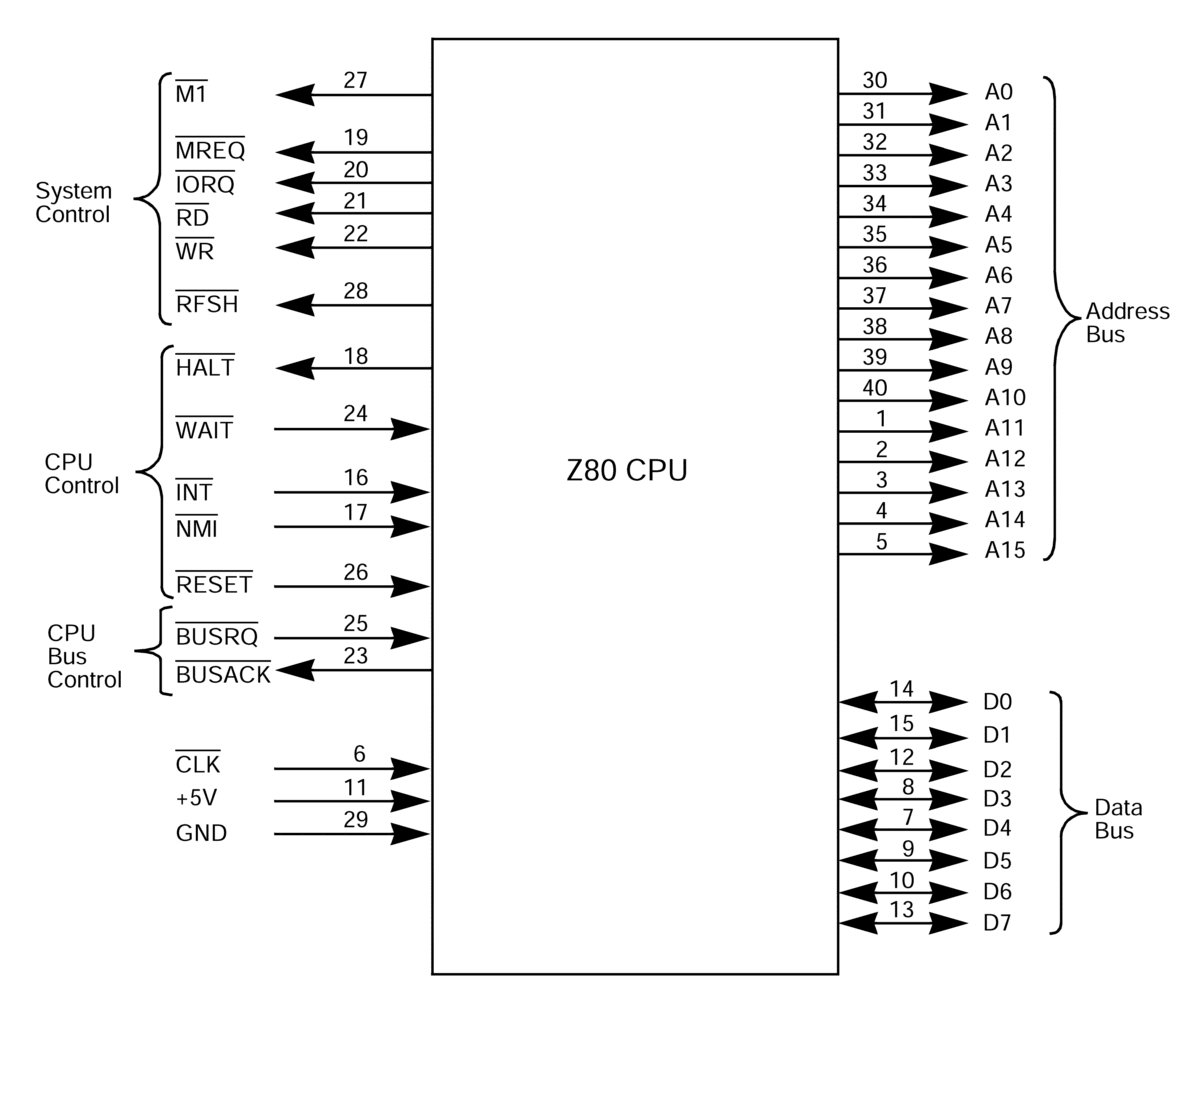
\includegraphics[width=0.5\textwidth]{images/z80.jpg}
    \caption{Microprocesor Z80.}
    \label{fig:z80}
\end{figure}

\subsubsection{Registrii}
\cite{ref:z80instructions}Procesorul are 10 registrii pe 8 biti,8 din care sunt pentru uz general, si 4 registrii pe 16 biti.
Rolul registrilor:
\begin{itemize}
    \item A,B,C,D,E,H,L sunt registrii de uz general pe 8 biti.
    \item F este un registru de flaguri.
    \item PC este un registru pe 16 biti care contine adresa instructiunii curente.
    \item SP este un registru pe 16 biti care contine adresa stivei.
    \item IX si IY sunt registrii pe 16 biti folositi pentru indexare.
    \item I este un registru pe 8 biti folosit pentru intreruperi.
    \item R este un registru pe 8 biti folosit pentru temporizare.
    \par \hspace{1em} \textit{Acesta este incrementat cu 1 la fiecare instructiune executata.}
    \item AF, BC, DE si HL sunt registrii de uz general pe 16 biti, fiecare fiind format de 2 registrii pe 8 biti.
\end{itemize}
Structura acestora se poate vedea si in Figura \cref{fig:z80registers}.
\begin{figure}[H]
    \centering
    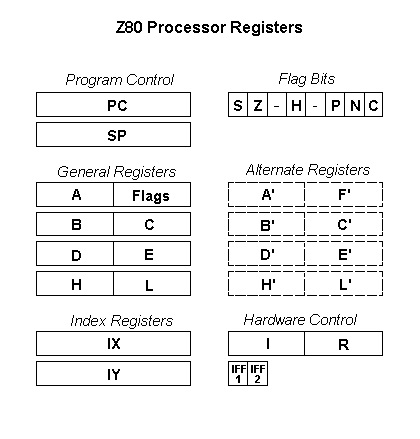
\includegraphics[width=0.5\textwidth]{images/z80registers.jpg}
    \caption{Structura registrii Z80. \cite{ref:z80registers}}
    \label{fig:z80registers}
\end{figure}

Registrul SP, varful stivei, este initializat cu 0xFFFF, valoarea acestuia scazand la instructiunile de PUSH si crescand la cele de POP

Registrul PC este initializat cu 0x0000.

Structura acestuia se poate vedea si in Tabela \cref{tab:z80flags}.
\begin{table}[h]
    \centering
    \begin{tabular}{|c|c|c|c|c|c|c|c|c|}
    \hline
    \textbf{Bit} & 7 & 6 & 5 & 4 & 3 & 2 & 1 & 0 \\
    \hline
    \textbf{Flag} & S & Z & F5 & H & F3 & P/V & N & C \\
    \hline
    \end{tabular}
    \caption{Z80 Flags}
    \label{tab:z80flags}
\end{table}

\subsubsection{Memorie}

Desi microprocesorul are magistrala de date pe 8 biti, acesta foloseste 16 biti pentru adresare. Datorita acestui lucru capacitatea maxima de memorie este de \(2^{16}=65536\) octeti. Aceasta zona de memorie de 64K poate fi separata intre \ac {ROM} si \ac {RAM} in functie de implementare.

Unele periferice in aceste sisteme sunt legate direct la memorie, acest lucru permitand microprocesorului sa comunice cu dispozitive externe prin simple scrieri si citiri din memorie.

Un exemplu de astfel de dispozitiv ar putea fi un ecran extern, fiecare pixel de pe acesta fiind reprezentat de o locatie in memorie, valoarea din aceasta specificand culoarea pixelului.

\subsubsection{Instructiuni}

Modelul oficial al \ac {Z80} contine 158 de instructiuni. Luand in considerare fiecare variatie a acestora, numarul total de instructiuni este de 696.
Instructiunile sunt impartite in 8 categorii principale:
\begin{itemize}
    \item Load si Exchange
    \item Transfer bloc de date si cautare
    \item Aritmetice si logice
    \item Rotiri/Shiftari
    \item Instructiuni la nivel de bit
    \item Jump/Call/Return
    \item \ac {IO}
    \item Control
\end{itemize}

Instructiunile de tip Load sunt cele care copiaza datele intern intre registrii sau intre registrii si memoria externa.
Toate aceste instructiuni specifica o locatie sursa de unde sa fie copiata valoarea si o destinatie unde sa fie copiata aceasta.
Locatia sursa nu este afectata de aceste instructiuni, aceasta fiind doar citita.
Exemple de asfel de instructiuni sunt cele care copiaza valoarea dintr-un registru in altul "LD A,B" sau cele care copiaza valoarea dintr-o locatie de memorie in registru "LD A,(HL)".

Instructiunile de tip exchange sunt cele care interschimba valorile dintre registrii.\\

Un set unic de instructiuni de transfer al blocurilor de date sunt include in \ac {Z80}.
Cu o singura instruciune, un bloc din memorie de orice marime poate fi mutat in orice alta locatie din memorie.
Aceste instructiuni sunt foarte folositoare in procesarea sirurilor de caractere.
Cu o singura instructiuni, un bloc intreg de de memorie de orice marime poate fi cautat dupa un anumit byte.
Cand valoarea este gasita sau se ajunge la sfarsitul blocului, instructiunea se opreste automat.
Instructiunile de acest tip permit intreruperile sa fie procesate in timpul executiei lor, astfel incat procesorul nu este blocat pentru perioade lungi de timp.\\

Instructiunile aritmetice si logice opereaza pe datele stocate in acumulator si alti registrii sau valori din memorie.
Rezultatul operatiei este stocat in acumulator.
De asemenea registrul de flaguri este actualizat in functie de rezultatul operatiei.\\

Rotate si Shift sunt grupuri de instructiuni care permit registrilor cat si valorilor din memorie sa fie rotite sau shiftate la stanga sau dreapta, cu sau fara carry.\\

Operatiunile la nivel de bit permit oricarui bit din acumulator, alt registru sau o locatie din memorie sa fie setat, resetat sau testat.\\

Jump, Call si Return sunt tipuri de instructiuni care transfera executia programului la o alta locatie din memorie.
Aceste instructiuni folosesc mai multe metode diferite de a transfera controlul programului.
Instructiunea Reset este un tip special de Call care permite saltul la doar 8 locatii diferite din memorie.
Alte instructiuni permit incarcarea Program Counter (PC) direct cu o valoare din memorie specificata de HL, IX sau IY.
Aceste instructiuni permit un nivel de control foarte inalt asupra executiei programului.\\

Instructiunile de \ac {IO} permit un spectru larg de transferuri de date intre microprocesor si dispozitivele externe.
O instructiune de acest tip foloseste ca port in transfer al doilea byte al instructiunii.
Alta instructiune permite portului sa fie specificat de registrul C.
Un avantaj mare in a folosi portul C, este ca permite unei functii sa fie refolosita pentru orice port.
Acest lucru nu ar fi posibil daca portul ar fi specificat de al doilea byte al instructiunii.
O buna caracteristica a acestor instructiuni este ca modifica automat flagurile in functie de rezultatul operatiei.
Din acest motiv nu este necesar sa se faca verificari suplimentare pentru a testa rezultatul operatiei. Exemplu: flagul de semn este setat daca rezultatul operatiei este negativ.\\

\ac {Z80} include instructiuni care sunt capabile sa mute blocuri intregi de date (pana la 256 byte) automata intre orice port \ac {IO} si memorie
Impreuna cu setul dual de registrii cu scop general, aceste instructiuni faciliteaza transferuri rapide de rate cu dispozitivele externe.\\

Instructiunile de control sunt instructiuni care controleaza mici aspecte ale microprocesorului.
Unele instructiuni de acest tip sunt cele care activeaza sau dezactiveaza intreruperile, sau cele care controleaza modul de raspuns la intreruperi.

\subsection{Emulator}
Un emulator reprezinta o metoda hardware sau software de a imita un alt tip de sistem de calcul, cum ar fi un procesor, consola sau chiar un intreg calculator.

In cazul acestui lucrari s-a ales un emulator software, acesta fiind mult mai accesibil.

Principala aplicatie a unui emulator este de a rula un program scris pentru o anumita arhitectura pe una complet diferita.

Acest lucru ajuta in mentenanta pe termen lung permitand inlocuirea componentei hardware vechi cu una mai noua fara a necesita software nou.

In cazul curent, deoarece \ac {Z80} este destul de vechi si procurarea acestuia a devenit o problema, in cazul in care microcontrolerul necesita inlocuirea, acesta va putea fi inlocuit cu un Raspberry Pi (sau o alternativa) ruland un emulator.

Pentru realizarea proiectului, emulatorul este necesar sa contina memoria, registrii, si logica necesara pentru decodarea si executarea instructiunilor.

Emularea se va face cat mai apropiat de un Z80 real, acest lucru fiind necesar pentru a asigura ca aplicatiile scrise pentru Z80 vor rula corect.
Pentru asigurarea calitatii si corectitudinii, toate instructiunile Z80 vor fi implementate, acestea fiind testate cu ajutorul unor teste unitare.

Emularea va functiona la nivel de instructiune, acest lucru permitand o monitorizare cat mai buna a executiei programului.
Utilizatorul va avea in fiecare moment control asupra executiei programului, acesta putand pune pauza executiei, modifica registrii sau vizualiza memoria.
Aceste facilitati ar trebui sa ofere un avantaj enorm in depanarea aplicatiilor scrise pentru Z80.
Un asemenea debugger ii va permite programatorului sa vada exact ce se intampla in fiecare moment al executiei programului.

Deoarece se vrea un nivel cat mai inalt de control, memoria emulatorului de asemenea va putea fi configurata.
Zone intregi de memori pot fi alocate ca fiind \ac {ROM} sau \ac {RAM}, sau chiar nealocate.
Deoarece codul va rula in emulator, in cazul accesarii unei zone de memorie nealocate, acest lucru va fi detectat si va fi notifica utilizatorul.

Pentru a simula dispozitivele externe, emulatorul va avea si un sistem de porturi \ac {IO}.
Porturile \ac {IO} in cazul emulatorului, vor fi legate la niste dispozitive virtuale care vor simula dispozitivele reale.
Aceste dispozitive virtuale vor fi configurabile de catre utilizator, acesta putand alege ce dispozitive sa fie simulate si ce porturi sa fie folosite.
Exemplu: Emulatorul va putea simula accesul la un ecran, tastatura sau chiar un dispozitiv de stocare.

O alta caracteristica pe care o va avea emulatorul este cea de extensibilitate.
Emulatorul va fi scris ca o librarie, acesta putand fi inclus in orice alt proiect scris in Rust.
Acest lucru va permite utilizatoriilor sa isi creeze propriile dispozitive compatibile cu emulatorul.
Exemplu: Un utilizator ar putea sa creeze un dispozitiv care sa simuleze un ecran cu o rezolutie mai mare


%\begin{multicols}{2}

%\begin{lstlisting}[language=C++]
%#include <iostream>
%using namespace std;
%
%int main() {
%    cout << "Hello, C++!" << endl;
%    return 0;
%}
%\end{lstlisting}
%\end{multicols}

\subsection{Decizie limbaj de programare}

In procesul de alegere a limbajului de programare, s-au luat in considerare mai multe aspecte, cum ar fi:
:qperformanta, documentatie si securitate.

Performanta este un aspect important, deoarece emulatorul va trebui sa ruleze cat mai fluid si cat mai apropiat de un Z80 real.
Un emulator eficient putand fi capabil sa ruleze in functie de nevoie chiar mai rapid.

Din aceasta cauza a fost preferat un limbaj compilat ce permite un control mai fin asupra memoriei si a resurselor.

Limbaje cum ar fi JavaScript si Python desi capabile, ar avea probleme in a mentine nivelul de performanta necesar unui astfel de emulator.

Un limbaj foarte folosit, mai ales pe embedded este C/C++, acesta fiind considerat a fi printre cele mai rapide.

Alt limbaj care a fost luat in considerare a fost Rust, acesta fiind un limbaj modern,
care oferta acelasi nivel de control si performanta ca C/C++, dar cu un sistem de tipuri mai sigur si mai usor de folosit.

Un mare avantaj al \ac {Rust} este sistemul sau de tipuri si de ownership,
acesta putand preveni multe buguri comune din C/C++ cum ar fi race conditions, memory leaks sau dereferentierea unui pointer null.

\begin{wrapfigure}{r}{0.4\textwidth}
    \centering
    
\includegraphics[width=0.4\textwidth]{images/rust_gear_logo.png}
    \caption{Logo Rust}
    \label{fig:rust-logo}
\end{wrapfigure}

In \ac {Rust} nu exista pointeri null, acest lucru fiind inlocuit de tipul Option<T>,acesta fiind un enum care poate fi Some(T) sau None.

Datorita nivelului ridicat de securitate adus de Rust,
\ac {DARPA} a lansat proiectul TRACTOR, acest proiect are ca tinta transformarea automata a codului C/C++ in Rust.

Un alt motiv din cauza carui \ac {Rust} a fost ales ca limbaj pentru proiect, este faptul ca acesta poate fi compilat cu usurinta in \ac {WASM},
acest lucru va permite rularea aplicatiei in orice browser web modern.

\subsection{Web}

In ultimii ani, aplicatiile web au devenit din ce in ce mai populare, acestea fiind usor de accesat si de folosit.
Un avantaj major al aplicatiilor web este faptul ca acestea pot rula pe orice dispozitiv care are un browser web.
Datorita avansarii rapide in tehnologie, acum se pot gasi pe piata frigidere si masini de spalat care au un browser web, lucru care ar fi fost greu de crezut acum 20 ani.

Un alt avantaj al aplicatiilor web este faptul ca acestea pot fi rulate fara a fi instalate, acest lucru fiind un avantaj major in cazul unui emulator.
Mare parte din emulatoarele existente necesita instalare, acest lucru fiind un inconvenient pentru utilizatorii care nu doresc sau nu pot sa faca acest lucru.
Deoarece aplicatia este ruleata din browser, utilizatorul nu risca sa descarce un virus, aplicatia web neavand access direct asupra calculatorului.
Un alt avantaj a creari unei aplicatii web este ca emulatorul va fi capabil sa ruleze pe orice arhitectura de procesor sau sistem de operare, atat timp cat acesta are un browser web modern.

Desi aplicatia web va fi capabila sa functioneze in mod standalone, complet offline, aceasta va putea fi integrata si in alte aplicatii web, oferind un nivel de control mai mare asupra acesteia.

In proiectul curent, va fi de asemenea folosit si un server pentru partea de backend. Desi nu este necesar, acesta este folosit pentru a oferi o experienta mai buna utilizatorului.
Anumite actiuni, cum ar fi compilarea codului C in cod Z80, nefiind posibile in browser, acestea fiind procesate de backend si apoi transmise inapoi catre client.

Contrar multor aplicatii web, aceasta nu va folosi javascript, singura parte de javascript fiind cea care incarca aplicatia \ac {WASM} in browser.
\ac {WASM} a fost ales deoarece este mult mai performant decat javascript, acesta fiind capabil sa ruleze cod mult mai rapid. De asemenea, deoarece fisierele ".wasm" sunt in format binar,
nu text precum javascript, acestea sunt mult mai compacte, ocupand mai putin spatiu si facilitand o incarcare mai rapida a aplicatiei.

\ac {Rust} a fost folosit ca limbaj de programare atat pentru frontend cat si pentru backend.
Folosirea aceluiasi limbaj de programare pe ambele parti, va facilita dezvoltarea si mentenanta aplicatiei.

Serializarea si deserializarea datelor reprezinta procesul prin care structuri de date complexe sunt convertite in format text sau binar, pentru a putea fi transmise pe retea sau salvate pe disk.
In cazul aplicatiei web, serializarea si deserializarea datelor este necesara pentru a putea transmite datele de la client la server si invers.
Pentru aceasta, se va folosi formatul JSON, acesta fiind un format des folosit pentru web, si foarte bine suportat de \ac {Rust}.
Datorita librariei de serializare/deserializare Serde, aceasta operatie este foarte usoara si rapida de realizat.
Toate structurile de date fiind serializabile/deserializabile cu modificari minime.
Acest lucru ne face foarte usoara transmiterea de obiecte intre server si client.

Serverul aplicatiei va avea access la randul sau la o baza de date, aceasta oferind functionalitatile extra doar utilizatorilor logati.
Pentru o securitate cat mai buna, parolele nu vor fi salvate direct in baza de date.
In schimb, acestea vor fi criptate folosind algoritmul de hashing argon2.
Aceasta metoda de criptare este una dintre cele mai sigure, aceasta fiind capabila sa reziste unor atacuri brute force chiar si pe cele mai puternice calculatoare.

De asemenea, un sistem de tokenuri va fi folosit pentru a autentifica utilizatorii.
Acest lucru va permite serverului sa stie daca un utilizator este logat sau nu, fara a fi nevoie de a trimite parola la fiecare request.
Un token unic este creat de server la fiegare logare, acesta fiind trimis inapoi si stocate in browser de catre client.
Server apoi la fiecare request va verifica daca tokenul este valid si daca este, va permite accesul la resursele protejate.

\subsection {Docker}

Docker\cite{ref:docker} este o platformă open-source destinată automatizării procesului de creare, livrare și rulare a aplicațiilor într-un mediu izolat numit container.
Scopul principal al Docker este de a facilita rularea aplicațiilor într-un mod reproductibil și portabil, indiferent de sistemul de operare gazdă.
\paragraph{Arhitectura Docker}

\begin{figure}[H]
\centering
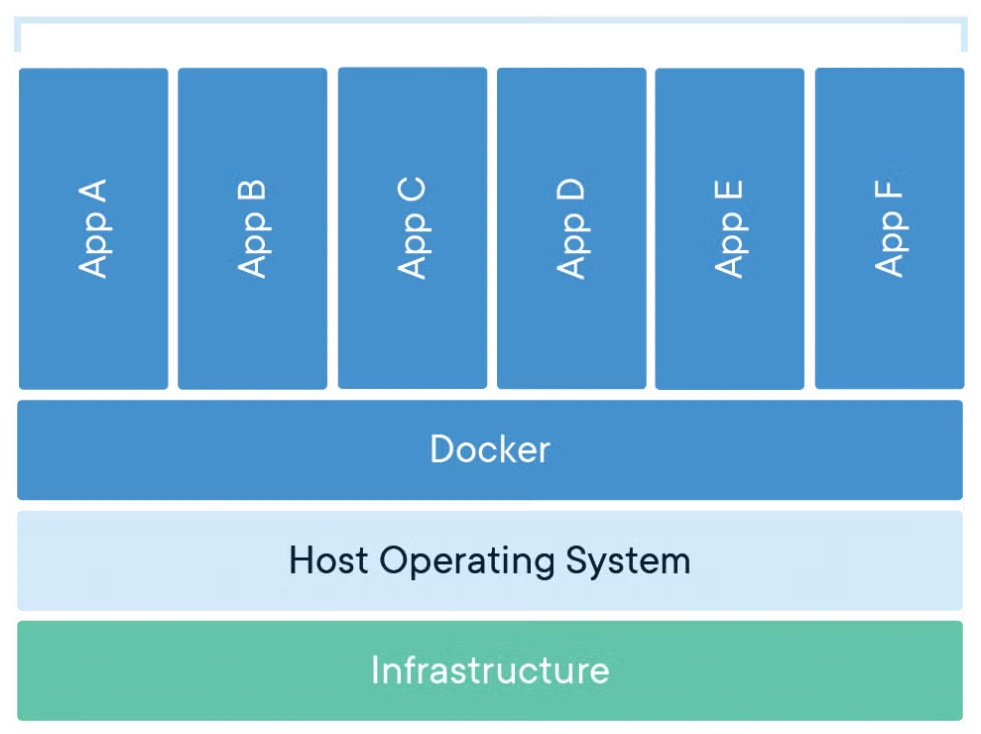
\includegraphics[width=0.6\textwidth]{images/dockerstructure}
\caption{Structura Docker.}
\label{fig:containerstructure}
\end{figure}

Un container Docker este o instanță rulabilă a unei imagini (image) Docker.
Imaginile sunt fișiere read-only ce conțin tot ceea ce este necesar pentru rularea unei aplicații: codul sursă, biblioteci, instrumente de sistem, fișiere de configurare și un runtime.
Aceste imagini sunt construite pornind de la un fișier special denumit \texttt{Dockerfile}, care conține instrucțiuni pas cu pas pentru configurarea mediului de execuție.

Fiecare container este izolat de celelalte și de sistemul gazdă, având propriile procese, rețele, sisteme de fișiere și spații de nume.
Spre deosebire de mașinile virtuale tradiționale, containerele împart același kernel al sistemului de operare, ceea ce le face mult mai eficiente în termeni de resurse.

Arhitectura Docker este compusă din mai multe componente-cheie:

\begin{itemize}
\item \textbf{Docker Engine} – serviciul care rulează pe sistemul gazdă și permite crearea, rularea și gestionarea containerelor.
\item \textbf{Imagini Docker (Docker Images)} – șabloane read-only folosite pentru a crea containere.
\item \textbf{Registrul Docker (Docker Registry)} – un sistem de tip repository pentru stocarea și partajarea imaginilor (ex: Docker Hub, GitHub Container Registry).
\item \textbf{Containere (Containers)} – instanțe izolate ale imaginilor, ce rulează aplicația propriu-zisă.
\item \textbf{Volume} – mecanism de persistență a datelor între mai multe rulări de containere.
\item \textbf{Rețele Docker (Docker Networks)} – oferă containerelor capacitatea de a comunica între ele sau cu lumea exterioară.
\end{itemize}

\paragraph{Avantajele utilizării Docker}

Docker oferă numeroase beneficii în dezvoltarea și livrarea aplicațiilor:

\begin{itemize}
\item \textbf{Portabilitate} – o aplicație containerizată poate fi rulată identic pe orice sistem cu Docker instalat, indiferent de mediul de execuție.
\item \textbf{Eficiență} – spre deosebire de mașinile virtuale, containerele au un overhead foarte redus și pornesc în câteva milisecunde.
\item \textbf{Izolare} – fiecare container rulează într-un spațiu izolat, ceea ce crește securitatea și stabilitatea aplicației.
\item \textbf{Scalabilitate} – Docker este integrat ușor cu sisteme de orchestrare precum Kubernetes sau Docker Swarm, permițând scalarea automată a aplicațiilor.
\item \textbf{Consistență} – mediile de dezvoltare, testare și producție pot fi standardizate, reducând riscul de erori cauzate de diferențe de configurație.
\end{itemize}

\paragraph{Docker în context DevOps și CI/CD}

În cadrul metodologiilor DevOps, Docker joacă un rol esențial în crearea unor pipeline-uri de livrare continuă (CI/CD).
De exemplu, codul sursă poate fi testat, construit și containerizat automat folosind instrumente precum GitHub Actions, GitLab CI, Jenkins sau Azure Pipelines.
Astfel, la fiecare commit, o nouă imagine poate fi generată, testată automat și livrată într-un mediu de staging sau producție.

\paragraph{Persistența datelor și comunicația între containere}

Pentru aplicațiile care necesită stocarea de date persistente, Docker oferă volume, care sunt directoare montate din exteriorul containerului.
Acestea permit salvarea datelor și după ce un container este oprit sau recreat.

Comunicarea între containere este posibilă prin rețele Docker dedicate.
Astfel, o aplicație web rulată într-un container poate comunica direct cu o bază de date aflată într-un alt container, fără a expune aceste servicii în exterior.

\begin{lstlisting}[language=docker,caption={Exemplu Dockerfile},label={lst:dockerfile}]
FROM rust:1.52
WORKDIR /usr/src/myapp
COPY . .
RUN cargo build --release
CMD ["cargo", "run"]
\end{lstlisting}

În exemplul din \cref{lst:dockerfile}, se construiește o imagine Docker pentru o aplicație Rust.
Aceasta este compilată în mod optimizat (\texttt{--release}) și apoi rulată automat la pornirea containerului.

\subsection{Version Control (Git)}

Controlul versiunilor este un sistem esențial în gestionarea codului sursă pe parcursul dezvoltării software. Acesta permite urmărirea modificărilor aduse fișierelor de-a lungul timpului, facilitând gestionarea mai multor versiuni ale unui proiect, colaborarea între dezvoltatori și asigurarea integrității și consistenței codului sursă.

Git este un sistem de control al versiunilor distribuit, creat de Linus Torvalds în 2005 pentru a sprijini dezvoltarea kernel-ului Linux. Spre deosebire de sistemele de control al versiunilor centralizate, Git oferă fiecărei instanțe a depozitului (repository) o copie completă a întregii istorii a proiectului. Acest lucru înseamnă că fiecare dezvoltator poate lucra în mod independent și local, iar modificările pot fi sincronizate ulterior cu depozitul central.

Principalele caracteristici ale Git sunt:

\begin{itemize}
\item \textbf{Sistem distribuit}: Fiecare dezvoltator are o copie completă a întregului proiect, inclusiv istoricul său, pe mașina locală. Aceasta permite lucrul offline și îmbunătățește performanța.
\item \textbf{Măcinarea și ramificarea ușoară}: Git permite crearea de ramuri (branches) ușor, care sunt esențiale pentru dezvoltarea paralelă a funcționalităților noi sau pentru testarea unor idei.
\item \textbf{Fazele fluxului de lucru}: Modificările sunt gestionate prin trei zone: Working Directory, Staging Area și Repository. Aceste zone permit dezvoltatorilor să adauge, să verifice și să stocheze modificările înainte de a le trimite în depozitul central.
\item \textbf{Performanță ridicată}: Git este extrem de rapid la operații comune, cum ar fi comiterea, schimbarea ramurilor sau unirea acestora.
\item \textbf{Securitate}: Git folosește un sistem de hash criptografic (SHA-1) pentru a verifica integritatea fișierelor și istoricului, protejând astfel datele împotriva corupției.
\end{itemize}

Un flux de lucru tipic cu Git implică următoarele etape:
\begin{enumerate}
\item \textbf{Clonarea depozitului}: Dezvoltatorul își clonează depozitul central pe mașina locală folosind comanda \texttt{git clone}.
\item \textbf{Crearea unei ramuri}: Dezvoltatorul creează o ramură de lucru pentru a dezvolta o caracteristică sau a rezolva o problemă.
\item \textbf{Comiterea modificărilor}: După ce au fost efectuate modificări, dezvoltatorul le adaugă în zona de stagiu (staging area) folosind comanda \texttt{git add}, iar apoi le salvează în depozitul local cu comanda \texttt{git commit}.
\item \textbf{Împingerea modificărilor}: După ce modificările sunt comise, acestea pot fi trimise la depozitul central folosind comanda \texttt{git push}.
\item \textbf{Îmbinarea modificărilor}: Dacă mai mulți dezvoltatori lucrează pe aceeași ramură, modificările lor pot fi combinate folosind comanda \texttt{git merge}.
\end{enumerate}

Comparativ cu alte sisteme de control al versiunilor, cum ar fi SVN (Subversion), Git oferă o mai mare flexibilitate și performanță. De exemplu, SVN este un sistem de control al versiunilor centralizat, ceea ce înseamnă că există un depozit central unde toate modificările sunt stocate. Git, pe de altă parte, este un sistem distribuit, permițând fiecărui dezvoltator să aibă o copie completă a întregului proiect, ceea ce îl face mai eficient în lucrul cu proiecte mari și echipe distribuite. Git este, de asemenea, mult mai rapid în gestionarea ramurilor și în combinarea modificărilor, fiind ideal pentru dezvoltarea de software agil.

\section{Implementare}
\subsection{Librarie emulator}
Implementarea emulatorului a fost realizata in limbajul de programare Rust, acesta fiind un limbaj modern, rapid si sigur. Deoarece se doreste o modularitate cat mai mare si posibilitatea de a integra proiectul in altele, nucleul emulatorului a fost realizat ca o librarie.
Libraria in sine va contine toate structurile necesare (Emulator, CPU, Io ...etc), cat si implementarea acestora. Impachetand nucleul emulatorului intr-o librarie permite utilizatorilor sa o extinda, cum ar fi sa isi creeze propri dispozitive virtuale sau sa adauge suport pentru alte procesoare.

\subsubsection{Structuri de date}

Pentru crearea emulatorului diferite structuri de date au fost create, fiecare avand rolul ei in cadrul emulatorului.

\paragraph{Emulator} Structura ce va coordona executia procesorului, memoriei si a sistemului IO

\begin{lstlisting}[language=Rust,caption={Structura Emulator},label={lst:emulator_struct}]
pub struct Emulator<T: Cpu> {
    pub memory: Memory,
    pub cpu: T,
    pub breakpoints: Vec<u16>,
    pub io: IO,
    pub cycle_counter: usize,
    pub instruction_counter: usize,
}
\end{lstlisting}

\subsubsection{Arhitectura}
\subsubsection{Testare automata}
\subsection{Interfata web}
\subsubsection{Frontend}
\subsubsection{Backend}
\subsection{Containerizare}

\section{Rezultate experimentale}
This is the conclusion.

\section{Contributii}
This is the conclusion.

\section{Bibliografie}
\printbibliography
\clearpage

\section{Anexe}
This is the conclusion.

\section{Planificarea activitatii}
This is the conclusion.


\end{document}
